\documentclass[11pt,a4paper]{scrartcl}
\usepackage[utf8]{inputenc}
\usepackage[ngerman]{babel}
\usepackage{amsmath}
\usepackage{amsfonts}
\usepackage{amssymb}
\usepackage{makeidx}
\usepackage{hyperref}
\usepackage{colortbl}
\usepackage{listings}
\usepackage{chngcntr}
\usepackage{upgreek}
\usepackage{pgfplots}
\pgfplotsset{compat = newest}
\usepackage{amsthm}
\usepackage{ulem}
\usepackage{tikz}
\usepackage{graphicx}
\usetikzlibrary{positioning}
\usepackage{tikz-network}
\usepackage[left=3cm,right=3cm,top=3cm,bottom=3cm]{geometry}

\usepackage[backend=biber, style=alphabetic]{biblatex}
\addbibresource{literature.bib}
\author{Roman Wetenkamp}
\title{Systemnahe Programmierung}
\subtitle{Technische Informatik II}

\newtheorem{note}{Bemerkung}
\newtheorem{definition}{Definition}
\newtheorem{satz}{Satz}
\newtheorem{theorem}{Theorem}
\newtheorem{lemma}{Lemma}
\newtheorem{example}{Beispiel}

\lstset{extendedchars=\true ,inputencoding=utf8}

\begin{document}
\vspace{3cm}
\maketitle
\begin{center}

\includegraphics[scale=0.7]{DHBW.jpg}
\end{center}
\pagebreak
\tableofcontents
\pagebreak
\section*{Vorwort}
Liebe Mitstudierende, \\\\
Systemnah Programmieren -- Klingt komplizierter als es ist. Vielleicht habt ihr euch schon einmal einen Elektronik-Adventskalender oder -baukasten schenken lassen, um damit herumzuspielen, einen Feuchtigkeitssensor für Blumenerde zu entwickeln oder die intelligente Wäscheklammer? In diesem Modul widmen wir uns genau mit diesem Gebiet, dem hardwarenahen Herumtüfteln an Mikrocomputern. \\\\
In diesem Skript notieren wir alles Relevante aus der Vorlesung, ergänzen es um ein paar Aufgaben und Anmerkungen und bereiten uns so auf die Klausur vor. Dieses Skript basiert auf der Vorlesung von Joachim Wagner an der DHBW Mannheim im Studiengang Informatik -- Cyber Security, die Passgenauigkeit für andere Dozierende oder Jahrgänge kann ich nicht beurteilen. \\\\
\textit{Viel Erfolg!}  \\
\begin{flushright}
Roman Wetenkamp \\
Mannheim, den \today
\end{flushright}  
\vfill
\paragraph{Fehlerfinden}
Mein Dank gilt folgenden Personen, die Fehler gefunden, korrigiert und so dieses Skript verbessert haben: 
\begin{itemize}
\item Daniel Riebel
\end{itemize}
\paragraph{Warnung}
Das Studium an einer Dualen Hochschule unterscheidet sich von dem Studium an Universitäten oder regulären Fachhochschulen insbesondere dadurch, dass aufgrund der Dualität von Theorie und Praxis meist nur die Hälfte der Zeit zur Vermittlung des Stoffes zur Verfügung steht (wenn dann auch intensiver). Daher gehen Sie bitte nicht davon aus, dass Sie dieses Skript ausreichend auf Klausuren in regulären Vollzeitstudiengängen vorbereitet!
\paragraph{Hinweis}
Dieses Dokument ist kein Vorlesungsmaterial, hat nicht den Anspruch auf {Voll}\-{ständigkeit} und enthält mit Sicherheit Fehler. Desweiteren ist es noch lange nicht vollendet (es ist infrage zustellen, ob es das je sein wird), und doch möchte ich Sie ermutigen, beizutragen! Jegliche Fehler, Probleme oder Anmerkungen können Sie mir gerne über das dazugehörige GitHub-Repository unter der URL \url{https://github.com/RWetenkamp/sysprog} zukommen lassen. Danke!
\pagebreak
\part{Einfache Ein-/Ausgabe-Prozesse}
\section{Einführung}
Systemnah zu programmieren bedeutet zuallererst, viele Ebenen der Abstraktion, die Betriebssysteme oder Virtualisierungen hinter sich zu lassen und zurückzukehren zu dem grundlegendsten Konzept der Computertechnik, dem Bit. \\
\begin{definition}
Ein Bit ist die kleinste Speichereinheit eines Computersystems. Der Wert eines Bits ist entweder \textbf{0} für \textbf{aus} oder \textbf{1} für \textbf{ein}. Sprechen wir von einem 8-Bit-Register, so bezeichnen wir damit acht einzeln adressierbare Werte, die jeweils auf 0 oder 1 gesetzt werden können. 
\[8 \text{ Bit } \widehat{=} 1 \text{ Byte }\]
\end{definition}

Sie werden in Ihren Programmen verschiedene Bitoperationen implementieren müssen, da die zugrundliegende Hardware zu großen Teilen aus Registern besteht, die sie auf diese Weise ansprechen können.
\begin{table}[h]
\centering
\begin{tabular}{|l|c|c|c|c|c|}
\hline
Bezeichnung & Symbol & C-Operatorsymbol & $a$ & $b$ & Ergebnis \\
\hline
Konjunktion & $\land$ & \texttt{\&} & 0 & 0 & 0 \\
&&&0 & 1 & 0 \\
&&&1 & 0 & 0 \\
&&&1 & 1 & 1 \\
\hline
Disjunktion & $\lor$ & \texttt{|} & 0 & 0 & 0 \\
&&&0 & 1 & 1 \\
&&&1 & 0 & 1 \\
&&&1 & 1 & 1 \\
\hline
XOR & $\oplus$ & \texttt{\^} & 0 & 0 & 0 \\
&&&0 & 1 & 1 \\
&&&1 & 0 & 1 \\
&&&1 & 1 & 0 \\
\hline
\end{tabular}
\caption{Übersicht über binäre Bitoperationen}
\end{table} \\

\begin{table}[h]
\centering
\begin{tabular}{|l|c|c|c|c|c|}
\hline
Bezeichnung & Symbol & C-Operatorsymbol & $a$ & Ergebnis \\
\hline
Negation & $\lnot$ & \texttt{~} & 0 & 1 \\
&&&1 & 0 \\
\hline
Linksverschiebung & &\texttt{<<} & 0000 & \texttt{1 << 1}: 0001, \texttt{1 << n}: 00...1...0 \\
\hline
Rechtsverschiebung & & \texttt{>>} & 1000 & \texttt{1 >> 1}: 0100, \texttt{1 << n}: 00...1...0 \\
\hline
\end{tabular}
\caption{Übersicht über unäre Bitoperationen}
\end{table}

Im folgenden Kapitel betrachten wir die verwendete Hardware und beginnen damit, die einzelnen Bestandteile und ihre Aufgaben zu erläutern. Wir werden jeweils anhand von Beispielprogrammen zeigen, wie die einzelnen Komponenten angesprochen und programmiert werden können. Die Programmiersprache hierfür ist C, in der Vorlesung wurde das {\glqq}Microchip Studio{\grqq} als IDE verwendet. Sie können es hier beziehen: 
\href{https://www.microchip.com/en-us/development-tools-tools-and-software/microchip-studio-for-avr-and-sam-devices}{Microchip Studio}

\section{Hardware}
Grundlegend ist Ihnen der Aufbau eines Computersystems sicherlich vertraut.
\begin{itemize}
\item Die \textbf{CPU} (Central Processing Unit), also der Prozessor, ist die zentrale Komponente, die die Befehle ausführt.
\item Während der Ausführung speichert die CPU Programmdaten im Arbeitsspeicher, dem \textbf{RAM} (Random Accessible Memory). Dieser Speicher wird nur zur Laufzeit genutzt und ist daher nicht persistent.
\item Ebenso gibt es einen Massenspeicher, eine Festplatte, auf der Daten persistent gespeichert werden und bei Bedarf gelesen/geschrieben werden.
\end{itemize}
Diese Grundstruktur gleicht im Wesentlichen dem \textsc{Von-Neumann-Prinzip} und ist sowohl auf klassische PCs anwendbar als auch auf Microcontroller, denen wir uns im Rahmen dieser Vorlesung widmen wollen.
\\
\begin{note}
Ein \textbf{Microcontroller} ist ein Minicomputer auf einem Chip. Er enthält einen Microprozessor und Speicher.
\end{note}
Ein solcher Microcontroller findet sich häufig auf Entwicklungsboards, wie z. B. der Arduino-Produktfamilie, die bereits aufgelötete Ports für weitere Komponenten enthalten. Derartige Boards gibt es zuhauf im Markt. Häufig sind die Unterschiede gering, da Arduino-Boards unter einer Open-Source-Lizenz stehen und somit von anderen ohne Weiteres kopiert werden dürfen. \\\\
Im Rahmen dieser Vorlesung arbeiten wir mit Arduino-Microcontrollern oder zu Arduino kompatiblen Äquivalenten. Die von uns verwendeten Boards enthalten allesamt folgenden Microprozessor:
\begin{center}
\textbf{ATMEL ATmega 328P}
\end{center}
Die Kenntnis des Microcontrollers ist unabdingbar für den weiteren Verlauf der Vorlesung. \\
Die Microcontroller Arduino Uno und Arduino Nano enthalten genannten Prozessor. Wir werden als Referenz jeweils den Arduino Uno verwenden.
\begin{figure}[h!]
\centering
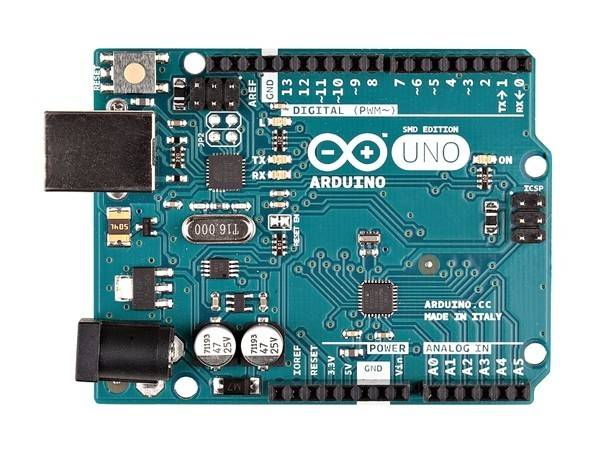
\includegraphics[scale=0.4]{uno.png}
\caption{Arduino Uno mit ATMEL ATmega328P}
\end{figure}
\paragraph{Aufbau}
Dieser Microcontroller enthält einige relevante Komponenten, die über einen Bus mit der CPU verbunden sind. Wir entnehmen diese dem folgenden Blockschaltbild.
\begin{figure}[h!]
\centering
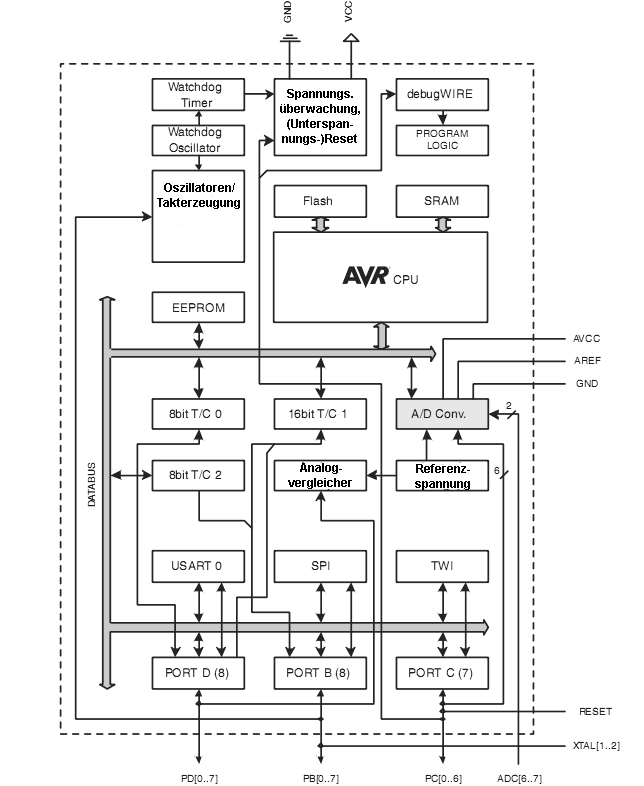
\includegraphics[scale=0.5]{b2-1.png}
\end{figure}
\begin{itemize}
\item \textbf{Flash} -- Der Flash-Speicher ist neben SRAM und EEPROM einer der drei Speichertypen. Der Flash-Speicher ist unveränderlich und kann lediglich von außen gebrannt werden. Hier wird das aktuelle Skript / Programm gespeichert.
\item \textbf{SRAM} -- Hierbei handelt es sich um einen winzig kleinen Arbeitsspeicher. Dieser Speicher ist nicht persistent und wird von der CPU während der Laufzeit verwaltet und verwendet.
\item \textbf{EEPROM} -- Dieser Speicher ist persistent und fungiert als {\glqq}Festplatte{\grqq}.
\item \textbf{Watchdog} -- Sollte der Chip nach einer gewissen Zeit kein Lebenssignal mehr senden, setzt der Watchdog den Microcontroller automatisch zurück.
\item \textbf{A/D Converter} -- Die Prozessoren der ATmega-Reihe können analoge Signale in digitale umwandeln. Dafür ist dieser Baustein zuständig.
\item \textbf{8/16bit T/C} -- Diese Bauteile sind Timer/Counter, die zur Prozesssteuerung genutzt werden können. Wir widmen uns diesen Bauteilen später.
\item \textbf{USART} -- Eine serielle Schnittstelle für diversen Datenverkehr ist der USART-Baustein.
\item \textbf{TWI} -- Die TWI-Schnittstelle kann für die Verknüpfung mehrerer Microcontroller untereinander genutzt werden.
\end{itemize}
Im Allgemeinen wird die Kommunikation mit jeder Hardware/CPU über I/O-Ports abgewickelt. 
\begin{note}
Gelegentlich kann es zu Verwirrung kommen, da sowohl internen I/O-Ports des Microcontrollers als auch die Anschlusspins für elektronische Bauteile als \textbf{Ports} bezeichnet werden. Im Kontext dieses Kurses bezeichnen wir letztere als {\glqq}Beinchen{\grqq}.
\end{note}
\paragraph{System} Der hier gezeigte Controller folgt der \textbf{RISC}-Architektur. RISC steht für {\glqq}Reduced Instruction Set Controller{\grqq}. Es hat sich gezeigt, dass mit einem im Vergleich zu Assembler reduzierten Befehlssatz ähnlich effizient, jedoch viel leichter dekodierbar und in der Regel schneller, gearbeitet werden kann. Der Microcontroller enthält von sich aus kein Betriebssystem. Wollen wir ein Programm ausführen, so müssen wir dieses speziell für diesen Microprozessor in einer hardwarenahen Programmiersprache wie Java oder C implementieren.
\section{Grundlegendes zur Programmierung}
Wir werden in dieser Vorlesung -- und damit auch in diesem Skript -- die Programmiersprache C verwenden. Um die benötigten Bibliotheken nutzen zu können, müssen die passenden Treiber installiert werden. Am einfachsten lässt sich dies durch die Arduino IDE und das zuvor erwähnte Microchip Studio realisieren. Das \textbf{Flashen}, also das Aufspielen der Programme auf das Board, erfolgt über USB.
\paragraph{Programmaufbau}
Wie Sie es von C gewohnt sein werden, unterscheiden wir \textbf{Programmzeilen} und \textbf{Präprozessordirektiven}. Die Befehle, die ausgeführt werden sollen, müssen Bestandteil der \texttt{main()}-Funktion des Programms sein.
\begin{note}
Jedes Programm, dass Sie flashen wollen, muss eine Endlosschleife enthalten! Andernfalls wird die Operation lediglich ein einziges Mal ausgeführt.
\end{note} 
Angewandt bedeutet dies:
\begin{lstlisting}[language=C]
#define F_CPU 16000000UL
#include <avr/io.h>

int main() {
	// Initialisierungen
	while(1) {
		// Hier koennen Sie Ihren Code platzieren	
	}
}
\end{lstlisting}
Sie erkennen die Definition der Konstante F{\_}CPU in der ersten Zeile. Hier legen wir fest, dass der Prozessor mit einem Takt von 16 MHz arbeitet.
\subsection{Register und Ports}
Unser Ziel ist es, verschiedene elektronische Bauteile an den Ports des Microcontrollers anzuschließen und mit diesem interagieren zu lassen. Dafür veranschaulichen wir uns zunächst die Pinbelegung des Boardes.
\begin{figure}[h!]
\centering
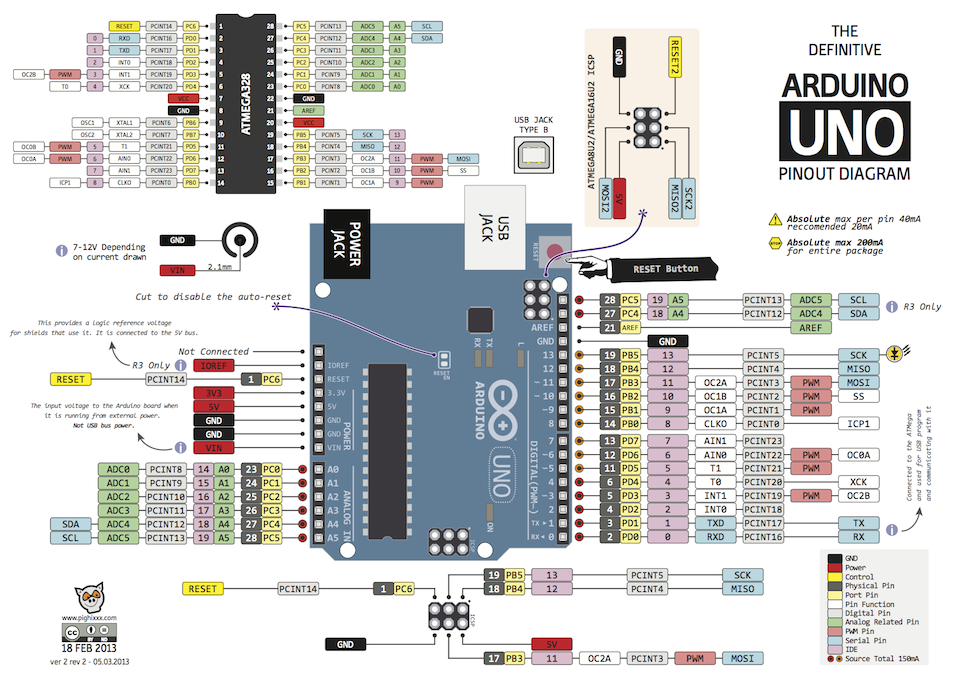
\includegraphics[scale=0.8]{pins.png}\label{pins}
\caption{Pinbelegungen des Arduino Unos}
\end{figure}
Von Relevanz für das nun folgende programmatische Ansprechen der Pins sind die hier gelb hinterlegten {\glqq}Port Pin{\grqq}-Belegungen, also beispielsweise der Port \textbf{PB5} an Pin 19 bzw. Onboard-IDE 13. Wir erkennen, dass es drei mal acht dieser Ports gibt, die Register PB (für Port B), PC und PD. Diese Ports nutzen wir -- wie angesprochen -- um zusätzliche Bauteile anzusprechen. \\\\
Für jeden dieser 24 Pins müssen wir festlegen, ob es sich um eine Input- oder Output-Port handelt. Diese Informationen halten wir im \textbf{DDR (Data direction register)} fest.
\paragraph{Programmzeilen} \quad
\begin{lstlisting}[language=C]
DDRB |= (1 << DDB5);					// (1)

DDRD |= (1 << DDD3) | (1 << DDD4) | (1 << DDD5);	// (2)

DDRD &= ~(1 << DDD2);					// (3)
\end{lstlisting}
\begin{itemize}
\item[(1)] Im Data Direction Register B verschieben wir eine 1 an die Stelle des fünften Bits, um Pin B5 als Ausgang zu definieren. Wir verwenden die Disjunktion, um andere, möglicherweise bestehende Eingaben, nicht zu überschreiben. Alternativ dazu ließe sich das Register selbstredend auch durch eine Angebe der Art \texttt{0b00100000} initialisieren, falls man beabsichtigt, nur das Bit 5 als Ausgang zu definieren.
\item[(2)] In dieser Zeile gehen wir ähnlich vor und initialisieren das DDR D. Nun soll jedoch nicht bloß ein einzelnes Bit initialisiert, sondern drei gleichzeitig, die wir gegenseitig disjunktiv verknüpfen.
\item[(3)] Nun bleibt noch, einen Pin wie hier als Eingang zu definieren. Da sich Nullen binär nicht schieben lassen, arbeiten wir hier mit der Negation der 1-Shift-Operation.
\end{itemize}
Im nächsten Kapitel betrachten wir die Möglichkeiten des Einlesens genauer, insbesondere behandeln wir dort Interrupts. \\\\
Mit der Definition des DDRs für die entsprechenden Bits ist die Hälfte getan. Wollen wir nun die Systemspannung von 5 V an einen spezifizierten Port anlegen, gehen wir analog vor:
\begin{lstlisting}[language=C]
PORTB |= (1 << PORTB5);			// einschalten
PORTB &= ~(1 << PORTB5);		// ausschalten
\end{lstlisting}
\subsection{Eingangssignale}
In vielen Schaltungen verwenden wir Taster und Schalter, um auf Benutzereingaben zu reagieren. Diese Bauelemente beeinflussen die Ströme, in dem eine Spannung erst bei Tastendruck anliegt oder dann nicht mehr. Der Microcontroller liest diese Spannungen nun aus und interpretiert sie entsprechend mit 0/1 (an/aus). Für dieses Verfahren gibt es zwei Varianten:
\begin{itemize}
\item \textbf{Polling} -- Hierbei wertet das Programm intervallbasiert die anliegende Spannung am Pin des Bauelements aus. Dieses Vorgehen ist ressourcenintensiv und daher nach Möglichkeit zu vermeiden.
\item \textbf{Interrupts} -- Effizienter hingegen ist es, wenn das Programm durch einen vordefinierten Interrupt unterbrochen wird. Dieses Verfahren wird im nächsten Kapitel ausführlicher behandelt.
\end{itemize}
Eine allgemeine Schwierigkeit beim Einlesen der Daten liegt aufgrund des \textbf{Prellens} vor. So verläuft der Spannungswechsel zwischen 0 und 5 V längst nicht so sauber, wie es wünschenswert ist. Stattdessen kann es bis zu 10 Sekunden dauern, bis ein klares Signal vorliegt,
 da elektromagnetische Spannungen und Wellen die gemessene Spannung verändern. Um diesem Phänomen zu begegnen, werden sogenannte \textbf{Pull-Up-Widerstände} eingesetzt, die dafür sorgen, dass die Spannung im nicht gedrückten Zustand {\glqq}hochgehoben{\grqq} wird und im Falle des Tastendrucks spürbar abfällt. Der Widerstand hat hierbei häufig den Wert $4.7 \text{ k}\Omega$.
\begin{figure}[h!]
\centering
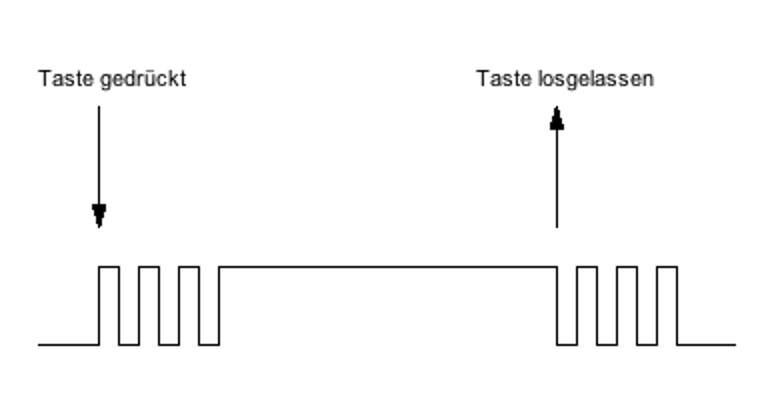
\includegraphics[scale=0.6]{prellen.png}
\caption{Prellen eines Tasters}
\end{figure}
\section{Programmbeispiele}
An dieser Stelle will ich die relevantesten Programme aus der Vorlesung abbilden, um sie reproduzierbar zu machen.
\subsection{Blinken}
Ein Standard-Beispiel, um zu testen, ob ein Arduino-Board funktionsfähig ist, ist das \textbf{Blink}-Beispiel. Wir wollen die Onboard-LED des Boards in einem vordefinierten Intervall zum Blinken bringen.
\paragraph{Schaltung} Für dieses Beispiel müssen keine weiteren Komponenten an das Board angeschlossen werden. Wir verwenden lediglich die bereits fest verlötete Onboard-LED.
\paragraph{Programm} \quad
\begin{lstlisting}[language=C]
/*
 * Blinken
 *	
 */ 

#define F_CPU 16000000UL	// Prozessortaktkonstante
#include <avr/io.h>		// Systembibliothek
#include <util/delay.h>		// Systembibliothek

int main(void)
{
	DDRB |= (1 << DDB5);		// initialisiert B5 als Ausgangspin
	PORTB |= (1 << PORTB5);		// legt Spannung an Port B5 an
	
	while (1) 
	{
		PORTB &= ~(1 << PORTB5);	// entzieht B5 die Spannung
		_delay_ms(500);			// Wartet 500 Millisekunden
		PORTB |= (1 << PORTB5);		// setzt B5 unter Spannung
		_delay_ms(500);
	}
}
\end{lstlisting}
\subsection{Tastendruck auslesen}
Nun wollen wir zwei Taster mittels Polling auslesen und bei die Onboard-LED bei Tastendruck ein- bzw. ausschalten.
\paragraph{Schaltung} Zusätzlich zum Entwicklungsboard benötigen wir nun zwei Taster, den wir auf einem Steckbrett befestigen und mit Port D2 und D3 des Boards verbinden. Der zweite Anschluss der Taster wird mit GND (Masse) verbunden. Bezogen auf obige Grafik handelt es sich dabei um die Pins 16, 17 und 20 (GND).
\paragraph{Programm} \quad
\begin{lstlisting}[language=C]
#include <avr/io.h>

int main(void)
{
	DDRD &= ~(1 << DDD2);	// D2 ist Eingabe
	DDRD &= ~(1 << DDD3);	// D3 ist Eingabe
	
	// Pull up
	PORTD |= (1 << DDD2) | (1 << DDD3);
	
	DDRB |= (1 << PORTB5);		// Onboard-LED ist Ausgabe
	PORTB &= ~(1 << PORTB5);	// Onboard-LED ist initial aus
	
    while (1) 
    {
    		// Auslesen der Taster
		if(! (PIND & (1 << DDD2))){
			// Einschalten der LED			
			PORTB |= (1 << PORTB5);
		}
		
		if(! (PIND & (1 << DDD3))){
			// Ausschalten der LED			
			PORTB &= ~(1 << PORTB5);
		}
    }
}

\end{lstlisting}
\section*{Aufgaben}
\begin{enumerate}
\item Nennen Sie die drei unterschiedlichen Arten von Speicher. Erläutern Sie die Unterschiede.
\item Erläutern Sie das Vorgehen, um eine weitere LED vom Board aus unter Spannung zu setzen.
\item Schließen Sie eine LED an Port B3 und einen Taster an Port D2 an. Entwickeln Sie ein Programm, das beim Druck des Tasters zwischen der Onboard-LED und der externen LED umschaltet.
\end{enumerate}
\part{Interrupts}
\section{Interrupts}
Die zweite Variante, um mit Eingaben umzugehen, sind Interrupts. \\
\begin{definition}
Unter einem Interrupt verstehen wir eine kurzfristige und unmittelbare Unterbrechung der Programmausführung, um einen kurzen, zeitlich kritischen Vorgang abzuarbeiten.
\end{definition}
\paragraph{Motivation}
Dem Kontext von Eingaben nähern wir uns durch folgende Betrachtungsweise:
Während wir beim Polling fortwährend überprüfen, ob eine Bedingung eingetreten ist -- wie z. B. ein Tastendruck -- und dann auf dieses Ereignis reagieren, operieren wir bei Interrupts anders. Wir melden an, dass wir bei einem bestimmten Ereignis unterbrochen werden wollen. Tritt dieses Ereignis nun ein, wird unsere Programmausführung unterbrochen und die Behandlung des Ereignisses wird ausgeführt. Auf diese Weise besteht keine Notwendigkeit mehr, ressourcenintensiv die Bedingung fortwährend zu überprüfen, sondern viel mehr ergeben sich Möglichkeiten der Nebenläufigkeit. 
\paragraph{Umsetzung}
Wenn wir erneut die Abbildung \ref{pins} betrachten, so finden wir dort den Ports PD2 und PD3 die Bezeichnungen \textbf{INT0} und \textbf{INT1}. Diese Pins sind die einzigen direkt geschalteten Interrupt-Ports. Eine Änderung der Spannung an diesen Pins triggert die Interrupt-Routinen, die wir im Folgenden implementieren werden. Neben diesen beiden Interrupt-Pins gibt es eine Zahl weiterer, die über ein Multiplexing-Verfahren adressiert werden können. Dies war jedoch nicht Teil der Vorlesung und wird daher an dieser Stelle ausgespart. 
\paragraph{Interrupttabelle}
Für jeden möglichen Interrupt muss zentral gespeichert sein, was nach Eintritt des selbigen abläuft. Dazu steht am Anfang des Flash-Speichers die \textbf{Interrupttabelle}. So befindet sich beispielsweise für den Interrupt INT0 ein Eintrag in der Tabelle, der einen Sprungbefehl der Form \texttt{JMP 1000} oder \texttt{RETI} beinhaltet. Letzteres steht für {\glqq}Return from Interrupt{\grqq} und referenziert die Rücksprungadresse zurück in das Hauptprogramm.
\paragraph{ISR (Interrupt Service Routine)} Wir implementieren in unserem Programm sogenannte ISRs, in denen der Code steht, den wir im Falle eines Interrupts an einem spezifizierten Pin ausführen. 
\begin{lstlisting}[language=C]
ISR (INT0_vect) {
	// Programmzeilen
}
\end{lstlisting}
Der Code in den ISRs sollte so klein wie möglich sein, da die Abarbeitung per se kritisch ist und keine Interrupts ineinander ausgelöst werden sollten. Daraus folgt auch, dass keine teuren Operationen in ISRs zu erfolgen haben.
\paragraph{Konfiguration}
Um Interrupts im Programm nutzen zu können und auf Eingaben zu reagieren, müssen wir -- auf gewohnte Art und Weise -- wieder bestimmte Registereinträge ändern.
\begin{itemize}
\item \textbf{EICRA} (External Interrupt Control Register A) -- Die Bits in diesem Register spezifizieren genauer, welche Änderungen der Spannung am Interrupt-Pin die ISR auslösen. Die genauen Einstellungen hierfür sind den Datenblättern der Microcontroller zu entnehmen. Möglich ist beispielsweise, dass nur bei steigenden bzw. fallenden Flanken reagiert wird oder generell bei jedem Pegelwechsel. 
\begin{table}[h!]
\centering
\begin{tabular}{|p{1cm}|p{1cm}|p{1cm}|p{1cm}|p{1cm}|p{1cm}|p{1cm}|p{1cm}|}
\hline
7 & 6 & 5 & 4 & 3 & 2 & 1 & 0 \\
\hline
-- & -- & -- & -- & ISC11 & ISC10 & ISC01 & ISC00 \\
\hline
\end{tabular}
\caption{EICRA}
\end{table}
Dabei spezifizieren ISC11 und ISC10 zusammen INT1 und ISC01 und ISC00 INT0.
\item \textbf{EIMSK} (External Interrupt Mask Register) -- In diesem Register werden die Interrupts {\glqq}scharf geschaltet{\grqq}. Nur wenn das Bit für INT0 hier auf 1 gesetzt wurde, reagiert das Programm tatsächlich auf einen Interrupt an Pin 1.
\begin{table}[h!]
\centering
\begin{tabular}{|p{1cm}|p{1cm}|p{1cm}|p{1cm}|p{1cm}|p{1cm}|p{1cm}|p{1cm}|}
\hline
7 & 6 & 5 & 4 & 3 & 2 & 1 & 0 \\
\hline
-- & -- & -- & -- & -- & -- & INT1 & INT0 \\
\hline
\end{tabular}
\caption{EIMSK}
\end{table}
\end{itemize}
\section{Programmbeispiel}
\subsection{Lichtschalter}
Wir wollen Interrupts nutzen, um die Onboard-LED des Entwicklungsboards über zwei Schalter ein- und auszuschalten.
\paragraph{Schaltung}
Wir benötigen erneut zwei Schalter, die wir auf einem Entwicklungsboard platzieren. Jeweils einen Kontakt der Schalter verbinden wir mit GND und einen der anderen mit INT0/INT1, also PD2 und PD3.
\paragraph{Programm}\quad
\begin{lstlisting}[language=C]
#include <avr/io.h>
#include <avr/interrupt.h>	// Systembibliothek

ISR (INT0_vect) {	// ISR fuer INT0
	PORTB = 0x00;	// Schaltet die Ports an B aus
}			

ISR (INT1_vect) {	// ISR fuer INT1
	PORTB = 0xff;	// Schaltet die Ports an B ein
}


int main(void)
{
	DDRB = 0xFF;		// Alle B-Ports werden Ausgaenge
	PORTB = 0xFF;		// Schaltet alle B-Ports ein 
	
	DDRD &= ~(1 << DDD2); 	// D2 wird Eingang
	PORTD |= (1 << PORTD2);	// An D2 wird Spannung angelegt
	DDRD &= ~(1 << DDD3);	// D3 wird Eingang
	PORTD |= (1 << PORTD3);	// An D3 wird Spannung angelegt
	
	EICRA |= (1 << ISC00);	// INT0 triggert bei Pegelwechsel
	EICRA |= (1 << ISC11);	// INT1 triggert bei Pegelwechsel
	EIMSK |= (1 << INT0);	// INT0 wird scharf
	EIMSK |= (1 << INT1);	// INT1 wird scharf
	
	sei();			// set enable interrupt
	
    while (1) 
    {
    }
}
\end{lstlisting}
\section*{Aufgaben}
\begin{enumerate}
\item Erläutern Sie, inwiefern der Einsatz von Interrupts gegenüber Polling vorteilsbehaftet ist.
\item Nennen Sie Anforderungen an ISRs.
\item Bauen Sie eine Schaltung mit zwei Tastern an INT0 und INT1 und einem Summer an einem Port aus B nach Wahl auf. Entwickeln Sie ein Programm, dass die Frequenz des Summers bei Tastendruck verdoppelt (starten Sie mit einer niedrigen Frequenz) und dem Summer sofort die Spannung entzieht, sollte der andere Taster gedrückt werden (ein Not-Aus-Schalter). Verwenden Sie dafür Interrupts.
\end{enumerate}
\end{document}
